%%chapter 6 (now 5), SA, by Lesley, modified 12.02
%% unified with "Stochastic Processes" on 4/2011.
%
%\input{header}
%
%\begin{document}
%
%% First page number
%\setcounter{page}{1}
%% PREVIOUS section number
%\setcounter{section}{4}
%% PREVIOUS subsection number
%\setcounter{subsection}{0}
%
%% ***********************************************************************
%\textsc{Reinforcement Learning \hfill Spring 2015$\;$ \\
%Lecture Notes \hfill Shie Mannor and Nahum Shimkin}
%\vspace{-18pt}
%\par
%\hrulefill
%% ***********************************************************************
%
%
%% {\large
%
%\section{The Stochastic Approximation Algorithm}

\newcommand{\midarrow}{\to}
\newcommand{\uu}{\underline}
\newcommand{\oo}{\overline}
\newcommand{\limn}{\lim_{n \to \infty}}
\newcommand{\limsupn}{\limsup_{n \to \infty}}

\section{Stochastic Processes -- Some Basic Concepts}

\subsection{Random Variables and Random Sequences}

Let $(\Omega,\cF,P)$ be a probability space, namely:
\begin{itemize}
\item $\Omega$ is the sample space.
\item $\cF$ is the event space. Its elements are subsets
of $\Omega$, and it is required to be a $\sigma$-algebra
(includes $\emptyset$ and $\Omega$; includes all countable union of its members;
includes all complements of its members).
\item $P$ is the probability measure (assigns a probability in [0,1] to each element
of $\cF$, with the usual properties: $P(\Omega)=1$, countably additive).
\end{itemize}

A random variable (RV) $X$ on $(\Omega,\cF)$
is a function $X:\Omega \to \reals$, with values $X(\omega)$.
It is required to be {\em measurable} on $\cF$,
namely, all sets of the form $\{\omega: X(\omega)\le a\}$ are
events in $\cF$.

A vector-valued RV is a vector of RVs. Equivalently, it is a
function $X:\Omega \to \reals^d$, with similar measurability requirement.

A {\em random sequence}, or a discrete-time {\em stochastic process},
is a sequence $(X_n)_{n\ge 0}$ of
$\reals^d$-valued RVs, which are all defined on the same probability space.

\subsection{Convergence of Random Variables}

A random sequence may converge to a random variable, say to $X$.
There are several useful notions of convergence:
\begin{enumerate}
\item
Almost sure convergence (or: convergence with probability 1):
$$
X_n \xrightarrow[a.s.]{} X  \quad \text{if} \quad P \{\lim_{n\to\infty} X_n =X \} = 1 \,.
$$
\item
Convergence in probability:
$$
X_n \xrightarrow[p]{} X \quad \text{if} \quad
\lim_{n\to\infty} P (|X_n - X| > \epsilon) =0\,,
\forall \epsilon >0\,.
$$
\item
Mean-squares convergence (convergence in $L^2$):
$$
 X_n \xrightarrow[L^2]{} X
\quad \text{if} \quad
E |X_n - X_\infty|^2 \to 0 \,.$$
\item
Convergence in Distribution:
$$ \text{$X_n \xrightarrow[Dist]{} X$ (or $X_n \Rightarrow X$)}
\quad \text{if} \quad
Ef(X_n) \to Ef(X)$$
for every bounded and continuous function $f$.
\end{enumerate}

\medskip

The following relations hold:
\begin{itemize}
\item[a.]
Basic implications: \ \ \
(a.s. or $L^2$) $\Longrightarrow$ $p$ $\Longrightarrow$ Dist
\item[b.]
Almost sure convergence is equivalent to
$$
\lim_{n\to\infty} P \{\sup_{k\geq n} |X_k - X| > \epsilon) = 0 \,,
\quad \forall \epsilon >0\,.
$$
\item[c.] A useful {\em sufficient} condition for a.s.\  convergence:
$$
\sum_{n=0}^{\infty} P(|X_n-X| > \eps) < \infty \,.
$$
\end{itemize}

\subsection{Sigma-algebras and information}

Sigma algebras (or $\sigma$-algebras) are part of the mathematical structure of
probability theory.
They also have a convenient interpretation as ''information sets", which
we shall find useful.

\begin{itemize}
\item
Define $\cF_X\dfn \sigma\{X\}$, the $\sigma$-algebra generated by the RV $X$.
This is the smallest $\sigma$-algebra that contains all sets of the
form $\{X\leq a\} \equiv \{\omega\in\Omega: X(\omega) \leq a\}$.
\item
We can interpret $\sigma\{X\}$ as carrying all the information in
$X$. Accordingly, we identify
$$
E(Z | X) \equiv E(Z | \cF_X)\,.
$$
Also, ``$Z$ is measurable on $\sigma\{X\}$"  is equivalent to:
$Z=f(X)$ (with the additional technical requirement that $f$ is a
Borel measurable function).
\item
We can similarly define $\cF_n = \sigma\{X_1,\dots, X_n\}$, etc. Thus,
$$
E(Z | X_1,\dots,X_n) \equiv E(Z | \cF_n)\,.
$$
\item
Note that $\cF_{n+1} \supset \cF_n$: more RVs carry more information,
leading $\cF_{n+1}$ to be finer, or ``more detailed"
\end{itemize}

\subsection{Martingales}
A \emph{martingale} is defined as follows.
\begin{definition}[\textbf{Martingale}]
A sequence $(X_k, \cF_k)_{k\ge 0}$
on a given probability space $(\Omega,\cF, P)$
is a martingale if
\begin{itemize}
\item[a.]
$(\cF_k)$ is a ``filtration'' -- an increasing sequence of
$\sigma$-algebras in $\cF$.
\item[b.]
Each RV  $X_k$ is $\cF_k$-measurable.
\item[c.]
$E(X_{k+1} | \cF_k) = X_k$\ \  (P--a.s.).
\end{itemize}
\end{definition}
\paragraph{Note:}
\begin{itemize}
\item
Property (a) is roughly equivalent to: 
``$\cF_k$ represents (the information in)
some RVs $(Y_0, \ldots, Y_k)$'',
and (b) then means:\ \
$X_k$  is a function of $(Y_0, \ldots, Y_k)$.
\item
A particular case is $\cF_n=\sigma\{X_1,\dots,X_n\}$
\ (a self-martingale).
\item
The central property is (c), which says that the conditional mean
of $X_{k+1}$ equals $X_k$. This is obviously
stronger than  $E(X_{k+1})=E(X_k)$.
\item
The definition sometimes requires also that $E|X_n|<\infty$,
we shall assume that below.
\item
Replacing (c) by $E(X_{k+1} | \cF_k) \geq X_k$ gives a {\em submartingale},
while $E(X_{k+1} | \cF_k) \leq X_k$ corresponds to a {\em supermartingale}.
\end{itemize}

\paragraph{Examples:}
\begin{itemize}
\item[a.]
The simplest {example} of a martingale is
$$
X_k = \sum_{\ell=0}^k \xi_\ell\,,
$$
with $\{\xi_k\}\;$ a sequence of 0-mean independent RVs, and
$\cF_k= \sigma (\xi_0, \ldots, \xi_k)$.
\item[b.]
$X_k=E(X|\cF_k)$, where $(F_k)$ is a given filtration and $X$ a fixed RV.
\end{itemize}

Martingales play an important role in the convergence analysis of
stochastic processes. We quote a few basic theorems
(see, for example: A.N. Shiryaev, {\it Probability,} Springer, 1996).

\begin{theorem}[\textbf{Martingale Inequalities}]

Let$(X_k, \cF_k)_{k\ge 0}$ be a martingale. Then for every $\la>0$ and $p\ge 1$
$$
P\left\{ \max_{k\le n} |X_k| \ge \la \right\} \le \frac{E |X_n|^p}{\la^p},
$$
and for $p>1$
$$
% E\left[(\max_{k\le n}|X_k|)^p \right] \le \textstyle{(\frac{p}{p-1})^p} E(|X_n|^p) \,.
E[(\max_{k\le n}|X_k|)^p ] \le \textstyle{(\frac{p}{p-1})^p} E(|X_n|^p) \,.
$$
\end{theorem}

\paragraph{Martingale Convergence Theorems}
\begin{theorem}[\textbf{Convergence with Bounded-moments}] Consider a martingale $(X_k, \cF_k)_{k\ge 0}$.
Assume that:\\
\hspace*{1in} $E|X_k|^q \le C$ for some $C<\infty$, $q \ge 1$ and all $k$.\\
Then
$\{X_k\}$ converges (a.s.) to a RV $X_\infty$ (which is finite w.p.\  1).
\end{theorem}
\begin{theorem}[\textbf{Positive Martingale Convergence}] If $(X_k, \cF_k)$ is
a \uu{positive}
martingale (namely $X_n \ge 0$), then $X_k$ converges (a.s.) to some RV $X_\infty$.
\end{theorem}

\begin{definition}[\textbf{Martingale Difference}]
The sequence $(\xi_k, \cF_k)$ is a {\em martingale difference} sequence if
property (c) is replaced by $E(\xi_{k+1}| \cF_k) = 0$.
\end{definition}
In this case we have:
\begin{theorem}[\textbf{Martingale Difference Convergence}] Suppose that for some $0 < q \le 2$,
$\sum_{k=1}^\infty \frac{1}{k^q} E (|\xi_k|^q | F_{k-1}) < \infty$ (a.s.).
Then $\limn \frac{1}{n} \sum_{k=1}^n \xi_k = 0$ (a.s.).
\end{theorem}

For example, the conclusion holds if the sequence $(\xi_k)$ is bounded,
namely $|\xi_k| \le C$ for some $C>0$ (independent of $k$).


\paragraph{Note:}
\begin{itemize}
\item
It is trivially seen that $(\xi_n\dfn X_n-X_{n-1})$ is a martingale difference
if $(X_n)$ is a martingale.
\item
More generally, for any sequence $(Y_k)$ and filtration $(\cF_k)$, where
$Y_k$ is measurable on $\cF_k$,
the following is a martingale difference:
$$
\xi_k \triangleq Y_k - E(Y_k | \cF_{k-1})\,.
$$
The conditions of the last theorem hold for this $\xi_k$ if either:\\
(i) $|Y_k | \le M$ $\forall k$ for some constant $M < \infty$,\\
(ii) or, more generally, $E(|Y_k|^q | \cF_{k-1}) \le M$ (a.s.) for some $q>1$ and
a finite RV $M$.\\
In that case we have
$$
\frac{1}{n} \sum_{k=1}^n \xi_k \,\equiv\, \frac{1}{n}
\sum_{k=1}^n ( Y_k - E (Y_k | \cF_{k-1})) \to 0 \quad \text{(a.s.)}
$$
\end{itemize}


\section{The Basic SA Algorithm}

The stochastic approximations (SA) algorithm essentially solves a system
of (nonlinear) equations of the form
$$
h(\theta) = 0,
$$
based on noisy measurements of $h(\theta)$.

More specifically, we consider a (continuous) function $h: \reals^d \to \reals^d$,
with $d\ge 1$, which depends on a set of parameters $\theta \in\reals^d$.
Suppose that $h$ is unknown. However, for each $\theta$  we can measure
$Y= h(\theta) + \om$, where $\om$ is some $0$-mean noise.
The classical SA algorithm (Robbins-Monro, 1951) is of the form
\begin{align*}
\theta_{n+1} & = \theta_n + \alpha_n Y_n \\
& = \theta_n + \alpha_n[h(\theta_n)
+ \om_n], \quad n \ge 0\,.
\end{align*}
Here $\alpha_n$ is the algorithm the step-size, or {\em gain}.

Obviously, with zero noise ($\om_n\equiv 0$) the stationary points of the algorithm
coincide with the solutions of $h(\theta)=0$.
Under appropriate conditions (on $\alpha_n$, $h$ and $\om_n$) the algorithm
indeed can be shown to converge to a solution of $h(\theta)=0$.

\paragraph{References:
}\begin{enumerate}
  \item H.~Kushner and G.~Yin, {\em Stochastic Approximation Algorithms and Applications},
Springer, 1997.

  \item V. Borkar, {\em Stochastic Approximation: A Dynamic System Viewpoint}, Hindustan, 2008.

  \item J. Spall, {\em Introduction to Stochastic Search and Optimization: Estimation, Simulation
and Control}, Wiley, 2003.
\end{enumerate}

\paragraph{Some examples of the SA algorithm:}

\begin{itemize}
\item[a.]
{\em Average of an i.i.d.\ sequence:}
Let $(Z_n)_{n \ge 0}$ be an i.i.d.\  sequence with mean $\mu = E(Z_0)$ and
finite variance.  We wish to estimate the mean.

The iterative algorithm
$$
\theta_{n+1} = \theta_n + \frac{1}{n+1} [Z_n - \theta_n]
$$
gives
$$
\theta_n = \frac{1}{n} \theta_0 + \frac{1}{n} \sum_{k=0}^{n-1} Z_k \to
\mu \text{\ \ (w.p.~1),\ \ \ by the SLLN} .
$$
This is a SA iteration, with $\alpha_n=\frac{1}{n+1}$, and
$Y_n = Z_n - \theta_n$.
% = (\mu - \theta_n) + (Y_n-\mu).
Writing $Z_n=\mu+\om_n$ ($Z_n$ is considered a noisy measurement of $\mu$,
with zero-mean noise $\om_n$), we can identify
$h(\theta) = \mu - \theta$.

\item[b.]
{\em Function minimization:} Suppose we wish to minimize a (convex) function $f(\theta)$.
Denoting $h(\theta) = - \nabla f(\theta) \equiv -\frac{\partial f}{\partial
\theta}$, we need to solve $h(\theta) = 0$.

The basic iteration here is
$$
\theta_{n+1} = \theta_n + \alpha_n [-\nabla f (\theta) + \om_n].
$$
This is a ``noisy" gradient descent algorithm.

When $\nabla f$ is not computable, it may be approximated by finite
differences of the form
$$
\frac{\partial f(\theta)}{\partial \theta_i} \approx
\frac{f(\theta+ e_i\delta_i) - f(\theta-e_i\delta_i)}{2\delta_i}\,.
$$
where $e_i$ is the $i$-th unit vector.
This scheme is known as the ``Kiefer-Wolfowitz Procedure''.
\end{itemize}

\paragraph{Some variants of the SA algorithm}
\begin{itemize}
\item
{\em A fixed-point formulation:}
Let $h(\theta) = H(\theta) - \theta$. Then
$h(\theta) = 0$ is equivalent to the fixed-point equation
$H(\theta) = \theta$,  and the algorithm is
$$
\theta_{n+1} = \theta_n + \alpha_n [H(\theta_n) - \theta_n + \om_n] =
(1-\alpha_n) \theta_n + \alpha_n [H(\theta_n) + \om_n]\,.
$$
This is the form used in the Bertsekas \& Tsitsiklis (1996) monograph.

Note that in the average estimation problem (example a.~above) we get
$H(\theta)=\mu$, hence $Z_n=H(\theta_n) + \om_n$.

\item
{\em Asynchronous updates:}
Different components of $\theta$ may be updated at different times and rates.
A general form of the algorithm is:
$$
\theta_{n+1} (i) = \theta_n(i) + \alpha_n(i) Y_n(i), \quad i=1, \dots, d
$$
where each component of $\theta$ is updated with a different gain sequence
$\{\alpha_n(i)\}$. These gain sequences are typically required to be
of comparable magnitude.

Moreover, the gain sequences may be allowed to be {\em stochastic},
namely depend on the entire history of the process up to the time of update.
For example, in the TD(0) algorithm $\theta$ corresponds to the estimated
value function
$\hat V=(\hat V(s),\,s\in S)$, and we can define $\alpha_n(s)=1/N_n(s)$,
where $N_n(s)$ is the number of visits to state $s$ up to time $n$.

\item
{\em Projections:}
It is often known that the required parameter $\theta$ lies in some set
$B\subset \reals^d$.\\
In that case we could use the projected iterates:
$$
\theta_{n+1} = \text{\it Proj}_B [\theta_n + \alpha_n Y_n]
$$
where $\text{\it Proj}_B$ is some projection onto $B$.

The simplest case is of course when $B$ is a box, so that the components
of $\theta$ are simply truncated at their minimal and maximal values.

If $B$ is a bounded set then the estimated sequence $\{\theta_n\}$ is guaranteed
to be bounded in this algorithm. This is very helpful for convergence analysis.

\end{itemize}


\section{Assumptions}

\paragraph{Gain assumptions}

To obtain convergence, the gain sequence needs to decrease to zero.
The following assumption is standard.

\paragraph{Assumption G1:}  $\alpha_n \ge 0$, and
\begin{align*}
\mathrm{(i)} \quad & \sum_{n=1}^\infty \alpha_n = \infty\\
\mathrm{(ii)} \quad& \sum_{n=1}^\infty \alpha_n^2 < \infty\,.
\end{align*}
A common example is  $\displaystyle{\alpha_n=\frac{1}{n^a}}$, with
$\frac{1}{2} < a \le 1$.

\paragraph{Noise Assumptions}

In general the noise sequence $\{\om_n\}$ is required to be ``zero-mean'',
so that it will average out.

Since we want to allow dependence
of $\om_n$ on $\theta_n$, the sequence $\{\om_n\}$ cannot be assumed
independent. The assumption below allows $\{\om_n\}$ to be a martingale
difference sequence.

Let
$$
\cF_{n-1} = \sigma \{ \theta_0, \alpha_0, \om_0, \cdots, \om_{n-1};
\theta_n, \alpha_n\}
$$
denote (the $\sigma$-algebra generated by) the history sequence up to
step $n$. Note that $\om_n$ is measurable on $\cF_n$ by definition of the latter.

\paragraph{Assumption N1:}
\begin{itemize}
\item[(a)]
The noise sequence $\{\om_n\}$ is a martingale difference sequence relative to the
filtration $\{\cF_n\}$, namely
$$
E(\om_n | \cF_{n-1}) = 0 \qquad \text{(a.s.)}.
$$
\item[(b)] For some finite constants $A,B$ and some norm $\|\cdot \|$ on $\reals^d$,
$$E(\| \om_n\|^2 | \cF_{n-1}) \le A + B \| \theta_n\|^2 \quad \text{(a.s.)},
\quad \forall n\ge 1\,.$$
\end{itemize}

\paragraph{Example:} Let $\om_n \sim N(0,\sigma_n)$, where $\sigma_n$
may depend on $\theta_n$, namely $\sigma_n = f(\theta_n)$.  Formally,
\begin{align*}
E(\om_n| \cF_{n-1}) & = 0\\
E(\om_n^2| \cF_{n-1}) & = f(\theta_n)^2,
\end{align*}
and we require that $f(\theta)^2 \le A+B\theta^2$.

\paragraph{Note:}
When $\{\theta_n\}$ is known to be bounded, then (b) reduces to
$$
E(\| \om_n\|^2 | \cF_{n-1}) \le C  \quad \text{(a.s.)} \quad
\forall n
$$
for some $C<\infty$.
It then follows by the martingale difference convergence theorem that
$$
\limn \frac{1}{n} \sum_{k=1}^n \om_k = 0 \quad \text{(a.s.)}.
$$
However, it is often the case that $\theta$ is not known to be bounded
{\em a-priori}.


\paragraph{Markov Noise:}
The SA algorithm may converge under more general noise
assumptions, which are sometimes useful. For example, for each fixed $\theta$,
$\om_n$ may be a {\em Markov chain} such that its long-term average is zero
(but $E(\om_n|\cF_{n-1}) \not= 0$). We shall not go into that generality here.

\section{The ODE Method}

The asymptotic behavior of the SA algorithm is closely related to the solutions
of a certain ODE (Ordinary Differential Equation), namely
$$
\frac{d}{dt}\theta(t)=h(\theta(t)),
$$
or $\dot{\theta}=h(\theta)$.

Given $\{\theta_n, \alpha_n\}$, we define a {\em continuous-time} process
$\theta(t)$ as follows.  Let
$$
t_n = \sum_{k=0}^{n-1} \alpha_k\,.
$$
Define
$$
\theta(t_n) = \theta_n\,,
$$
and use linear interpolation in-between the $t_n$'s.

Thus, the time-axis $t$ is rescaled according to the gains $\{\alpha_n\}$.

\begin{center}
\scalebox{.7}{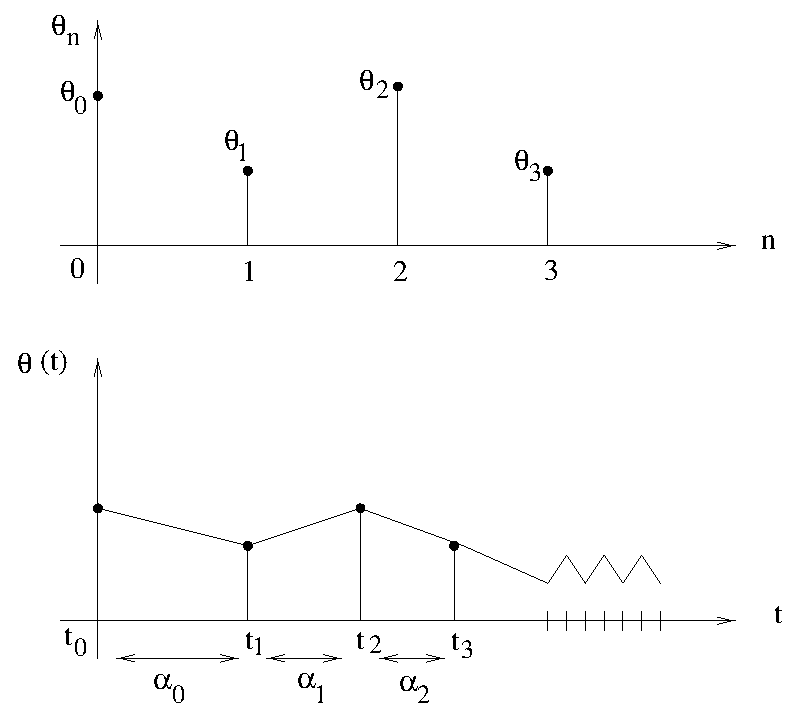
\includegraphics{figures/ch6_fig1a.eps}}
\end{center}


Note that over a fixed $\Delta t$, the ``total gain'' is approximately
constant:
$$
\sum_{k\in K(t, \Delta t)} \alpha_k \simeq \Delta t\,,
$$
where $K(t,\Delta t) = \{k: t \le t_k < t+ \Delta t\}$.

Now:
$$
\theta(t+\Delta t) = \theta(t) + \sum_{k\in k(t, \Delta t)} \alpha_k [h(\theta_n)
+\om_n] \,.
$$
\begin{itemize}
\item
For large $t$, $\alpha_k$ becomes small and the summation is over many
terms; thus the noise term is approximately ``averaged out'':
$\sum \alpha_k \om_k \to 0$.
\item
For small $\Delta t$, $\theta_k$ is approximately constant over $K(t, \Delta t):
h(\theta_k) \simeq h(\theta(t))$.
\end{itemize}
We thus obtain:
$$
\theta(t+\Delta t) \simeq \theta(t) +\Delta t\cdot h (\theta(t))\,.
$$
For $\Delta t \to 0$, this reduces to the ODE:
$$
\dot \theta(t) = h(\theta(t))\,.
$$

\medskip

To conclude:
\begin{itemize}
\item
As $n\to\infty$, we ``expect'' that the estimates
$\{\theta_n\}$ will follow a trajectory of the ODE $\dot\theta=h(\theta)$
(under the above time normalization).
\item
Note that the stationary point(s) of the ODE are given by
$\theta^*:\;\; h(\theta^*) = 0$.
\item
An obvious requirement for $\theta_n \to \theta^*$ is
$\theta(t) \to \theta^*$
(for any $\theta(0)$).
That is: $\theta^*$ is a {\em globally asymptotically stable} equilibrium of
the ODE.

This may be viewed as a necessary condition for convergence of
$\theta_n$. It is also sufficient under additional assumptions on
$h$ (continuity, smoothness), and boundedness of $\{\theta_n\}$.
\end{itemize}

% \uu{A Remark on Asynchronous Algorithms}:\quad
% When the stepsize is different for each component of $\theta$, the
% approximating ODE is more involved -- the relative rates should enter
% explicitly.
% Still, there exist specifc results that related
% the above ``synchronous'' ODE to the convergence of the
% asynchronous SA algorithm.


\section{Some Convergence Results}

A typical convergence result for the (synchronous) SA algorithm is the following:

\begin{theorem}\label{thm:SA_1}
Assume G1, N1, and furthermore:
\begin{itemize}
\item[(i)]
$h$ is Lipschitz continuous.
\item[(ii)]
The ODE $\dot\theta=h(\theta)$ has a unique equilibrium point $\theta^*$, which
is globally asymptotically stable.
\item[(iii)]

The sequence $(\theta_n)$ is bounded (with probability 1).
\end{itemize}
Then $\theta_n\to\theta^*$ (w.p.~1), for any initial conditions $\theta_0$.
\end{theorem}


\paragraph{Remarks:}
\begin{itemize}
\item[1.]
More generally, even if the ODE is not globally stable, $\theta_n$ can be shown to converge
to an {\em invariant set} of the ODE (e.g., a limit cycle).
\item[2.]
Corresponding results exist for the asynchronous versions, under suitable
assumptions on the relative gains.
\item[3.]
A major assumption in the last result in the boundedness of $(\theta_n)$.
In general this assumption has to be verified independently. However, there
exist several results that rely on further properties of $h$ to deduce
boundedness, and hence convergence.
\end{itemize}


The following convergence result from B.~\&T.~(1996) relies on
 \uu{contraction} properties of $H$, and applies to the
asynchronous case.
It will directly apply to some of our learning algorithms.
We start with a few definitions.

\begin{itemize}
\item
Let $H(\theta) = h(\theta) + \theta$, so that $h(\theta) = H(\theta) - \theta$.
\item
Recall that $H(\theta)$ is a {\em contraction operator} w.r.t.\ a norm
$\|\cdot\|$ if
$$
\| H(\theta_1) - H(\theta_2)\| \le \alpha \| \theta_1 - \theta_2\|
$$
for some $\alpha < 1$ and all $\theta_1, \theta_2$.
\item
$H(\theta)$ is a {\em pseudo-contraction} if the same holds for a
fixed $\theta_2=\theta^*$.
It easily follows then that $\theta^*$ is a unique fixed point of $H$.
\item
Recall that the {\em max-norm} is given by
$\|\theta\|_\infty = \max_i |\theta(i)|$.
The {\em weighted} max-norm, with a weight vector $w$, $w(i) > 0$, is given by
$$
\|\theta\|_w = \max_i \left\{ \frac{|\theta(i)|}{w(i)}\right\} 
\,.
$$
\end{itemize}

\begin{theorem}[Prop. 4.4. in B.\&T.]\label{thm:SA_2}
Let
$$
\theta_{n+1}(i) = \theta_n(i) + \alpha_n (i)  [H(\theta_n) - \theta_n +
\om_n]_i\,, \quad i=1, \cdots, d\,.
$$
Assume N1, and:
\begin{itemize}
\item[(a)]
Gain assumption: $\alpha_n(i) \ge 0$, measurable on the ``past'', and satisfy
$$
\sum_n \alpha_n(i) = \infty, \quad \sum_n \alpha_n(i)^2 < \infty \quad
\text{(w.p. 1)}\,.
$$
\item[(b)]
$H$ is a pseudo-contraction w.r.t.\ some weighted max-norm.
\end{itemize}
Then $\theta_n \to \theta^*$ (w.p.\  1), where $\theta^*$ is the unique fixed point
of $H$.
\end{theorem}



\paragraph{Remark on ``Constant Gain'' Algorithms}

As noted before, in practice it is often desirable to keep a non-diminishing
gain.
A typical case is $ \alpha_n(i)\in [\uu\alpha, \oo{\alpha}]$.

Here we can no longer expect ``w.p.\   1'' convergence results.  What can be
expected is a statement of the form:
\begin{itemize}
\item
For $\oo\alpha$ small enough, we have for all $\eps > 0$
$$
\limsupn P (\|\theta_n - \theta^* \| > \eps) \le b(\eps) \cdot
\oo\alpha\,,
$$
with $b(\eps) < \infty$.
\end{itemize}

This is related to ``convergence in probability'', or ``weak convergence''.
We shall not give a detailed account here.

%\section{Gain Selection}
%
%The choice of the gain sequence $(\alpha_n)$ can have drastic effect on the speed of
%convergence. Over the years there have been many suggestions for possible choices,
%which we briefly describe. The discussion is informal,
%under appropriate assumptions on the noise sequence. For more details
%see the book by Spall.
%
%{\em a. Asymptotic Optimality}
%
%Suppose we wish to minimize the asymptotic variance:
%$$ \lim_{\to\infty} E(\theta_n - \theta^*)^2 \.$$
%An optimal choice in this sense is $\alpha_n = \frac{1}{n}$ (pure averaging).
%The asymptotic variance can then be computed using the Central Limit Theorem (CLT).
%
%More precisely, for  $\alpha_n = \frac{a}{n^b}$, $b<2$, we get
%$$
%n^{\frac{b}{2}} (\theta_n -\hat{\theta}) \to_{distr.} N(0,\Sigma) \,,
%$$
%i.e., $\theta_n \sim \theta^* +\frac{1}{n^{\frac{b}{2}} \Sigma$, where
%$\Sigma$ is a fixed matrix (which depends on $a$). \\
%The best rate is obtained for $b=1$. \\
%$\Sigma$ is minimized by the choice of {\em matrix} gains: $a=H(\theta^*)^{-1}$,
%where $H(\theta) = \frac{\partial h(\theta)}(\partial \theta}$ is the Hessian
%matrix.
%
%{\em Averaging} A problem with the above choice is that the function $h$
%(hence the Hessian) are not known in advance. Also the gain sequence may
%decay too fast at the initial stage. An alternative that obtains the
%optimal asymptotic rate is the averaging scheme proposed by
%Polyak and Juditsky (1992):
%
%1. Compute $\theta_n$ with any gain sequence $\alpha_n$ that satisfies the
%usual conditions, and in addition: $\frac{\alpha_{n+1}}{\alpha_n} =1 - o(\alpha_n)$.
%For example, $\alpha_n = \frac{a}{n^b}$ with $0.5<\beta <1$, $a>0$.
%
%2. Take the average:   $\bar{\theta} = \frac{1}{n} \sum_{k=1}^n \theta_k$.
%
%Then $\bar{theta}_n$ has the optimal asymptotic convergence rate.

%{\em b. Heuristics}
%
%The aboce
%
%e slow convergence in the initial phase.
%Once solution is to start with another schedule (see the heuristics below) and then
%revert to $\frac{1}{n}$ for "fine tuning'' in the final stage.
%
%\end{document}
